\begin{figure}[t]
\centering
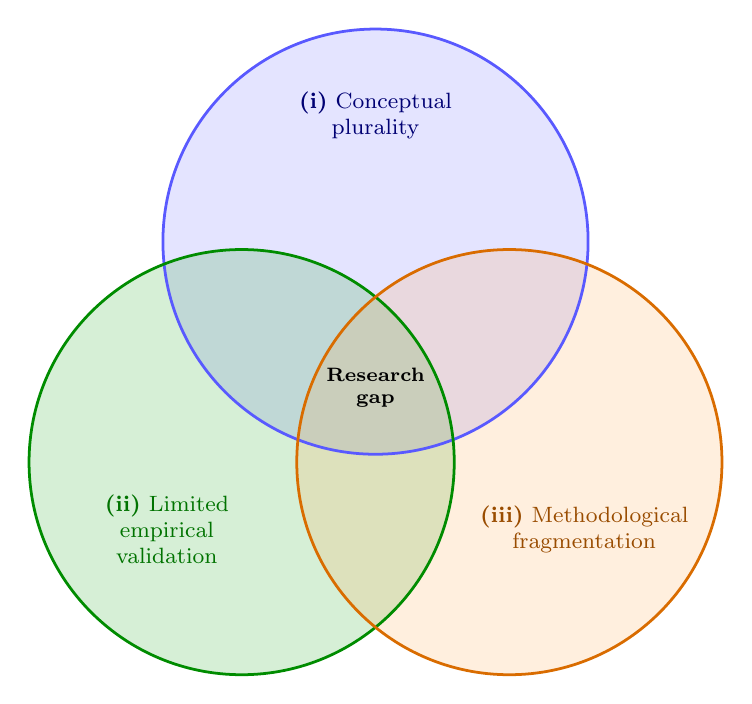
\begin{tikzpicture}[font=\footnotesize]

% ---- three deficit circles ----
\def\R{2.7}
\coordinate (Ci) at (0,1.5);      % (i)  conceptual plurality
\coordinate (Cii) at (-1.7,-1.3); % (ii) limited empirical validation
\coordinate (Ciii) at (1.7,-1.3); % (iii) methodological fragmentation

\begin{scope}[fill opacity=0.16]
  \fill[blue!65]        (Ci)   circle (\R);
  \fill[green!60!black] (Cii)  circle (\R);
  \fill[orange!80]      (Ciii) circle (\R);
\end{scope}
\draw[blue!65,line width=1pt]        (Ci)   circle (\R);
\draw[green!55!black,line width=1pt] (Cii)  circle (\R);
\draw[orange!85!black,line width=1pt](Ciii) circle (\R);

% ---- short labels in the solo lobes ----
\node[blue!45!black,align=center]    at (0,3.1)    {\textbf{(i)} Conceptual\\plurality};
\node[green!45!black,align=center]   at (-2.65,-2.15) {\textbf{(ii)} Limited\\empirical\\validation};
\node[orange!60!black,align=center]  at (2.65,-2.15)  {\textbf{(iii)} Methodological\\fragmentation};

% ---- the gap at the triple intersection ----
\node[align=center,font=\scriptsize\bfseries] at (0,-0.35)
  {Research\\gap};

\end{tikzpicture}
\caption{\textbf{The research gap as the intersection of three deficits.}
Resilience research is held back by three interlocking deficits:
\textbf{(i)} conceptual plurality without operational convergence,
\textbf{(ii)} limited empirical validation of adaptive performance, and
\textbf{(iii)} methodological fragmentation across domains. Each is individually
surmountable; it is their \emph{intersection} that defines the gap this review
targets---resilience can be declared but not evaluated, because the field
simultaneously lacks a shared construct (i), cumulative evidence (ii), and
transferable measures (iii). The Enactment--Scope framework and the agenda of
Section~\ref{sec:RD} are organized to close that overlap.}
\label{fig:venn_gaps}
\end{figure}
